% ------------------------------------------------------------------------------
% Palestra: Mecanismos para controle de variabilidades em aplica��es para Android
% Autores:
%     Adorilson Bezerra <adorilson@gmail.com>
% Licen�a Creative Commons Atribui��o 3.0. 
% Voc� pode usar e alterar este documento, 
% mas deve obrigatoriamente citar a autoria. 
% ------------------------------------------------------------------------------

\documentclass{beamer}

% ------------------------------------------------------------------------------
\usepackage[latin1]{inputenc}
\usepackage[brazil]{babel}
\usepackage{graphicx}
\usepackage{beamerthemesplit}
\usepackage{ae}
\usepackage{alltt}
\usepackage{pslatex}
% ------------------------------------------------------------------------------

\usecolortheme{beaver}

% ------------------------------------------------------------------------------
\title[Mecanismos para controle de variabilidades em aplica��es para Android]
{
    Mecanismos para controle de variabilidades em aplica��es para Android
}
\subtitle{}
\author[Adorilson Bezerra]
{
    Adorilson Bezerra
}
\institute{Universidade Federal do Rio Grande do Norte\\Departamento de Inform�tica e Matem�tica Aplicada}
\date{\today}
%\logo{
\includegraphics[scale=0.2]{img/android}}
% ------------------------------------------------------------------------------

\begin{document}

% ------------------------------------------------------------------------------
\frame{\titlepage}
% ------------------------------------------------------------------------------

\section{Introdu��o}
    \frame
    {
        \frametitle{Variabilidades em aplica��es para Android}
        \begin{itemize}
            \item Vers�o da API
            
            \item Dispositivos com ou sem sensores
            \item Gr�ficos 2D ou 3D
            \item Mecanismo de intera��o
            \item Pacote de compatibilidade
            \item Vers�o da OpenGL ES
            \item Android NDK
            
            \item Tamanhos e densidade das telas
            \item L�nguas internacionais
        \end{itemize}
    }
\section{Desenvolvimento}
    \frame
    {
        \frametitle{Vers�o da API}
        \begin{itemize}
            \item Reflex�o
        \end{itemize}
        \begin{figure}[t]
		    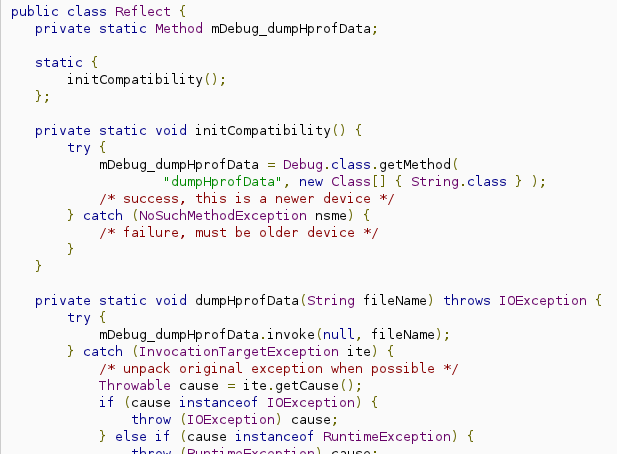
\includegraphics[scale=0.5]{img/reflect1.png}
		\end{figure}
    }
    \frame
    {
        \frametitle{Vers�o da API}
        \begin{figure}[t]
		    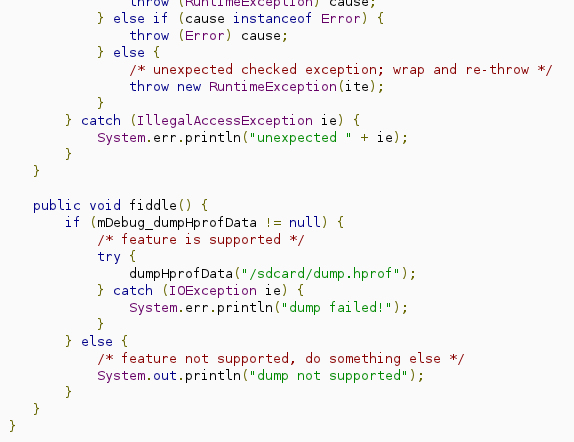
\includegraphics[scale=0.5]{img/reflect2.png}
		\end{figure}
    }
    \frame
    {
        \frametitle{Vers�o da API}
        \begin{itemize}
            \item Classe wrapper
        \end{itemize}
        \begin{figure}[t]
		    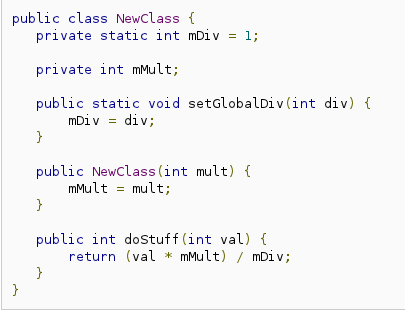
\includegraphics[scale=0.5]{img/wrapper1.png}
		\end{figure}
    }
    \frame
    {
        \frametitle{Vers�o da API}
        \begin{figure}[t]
		    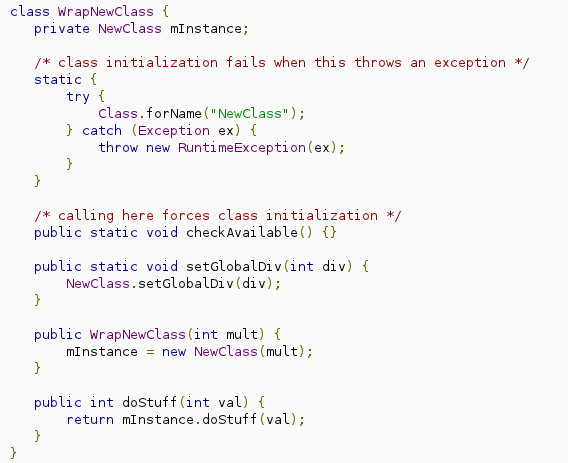
\includegraphics[scale=0.5]{img/wrapper2.png}
		\end{figure}
    }
    \frame
    {
        \frametitle{Vers�o da API}
        \begin{figure}[t]
		    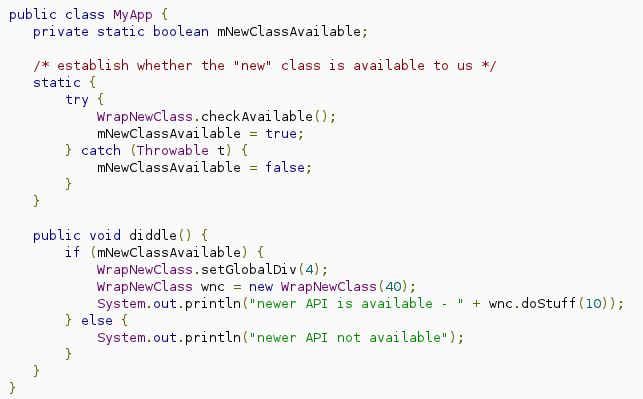
\includegraphics[scale=0.5]{img/wrapper3.png}
		\end{figure}
    }
    \frame
    {
        \frametitle{Vers�o da API}
        \begin{itemize}
            \item Checando vers�o exata em tempo de execu��o
        \end{itemize}
        \begin{figure}[t]
		    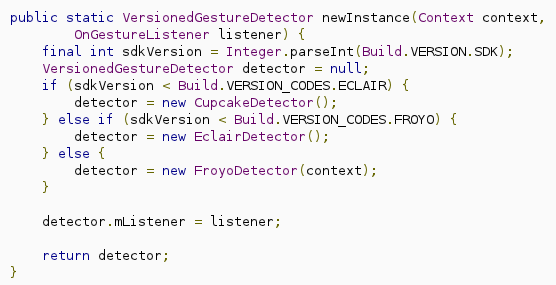
\includegraphics[scale=0.5]{img/versao.png}
		\end{figure}
    }
    \frame
    {
        \frametitle{Mesmo(s) mecanismo(s) anterior(es)}
        \begin{itemize}
            \item Dispositivos com ou sem sensores
            \item Gr�ficos 2D ou 3D
            \item Mecanismo de intera��o
            \item Pacote de compatibilidade
            \item Vers�o da OpenGL ES
            \item Android NDK
        \end{itemize}
        \begin{quote}
            A API fornece o m�todo PackageManager.hasSystemFeature()
        \end{quote}
    }
    \frame
    {
        \frametitle{S�o transparentes para o desenvolvedor}
        \begin{itemize}
            \item Tamanhos e densidade das telas
            \item L�nguas internacionais 
        \end{itemize}
        \begin{figure}[t]
		    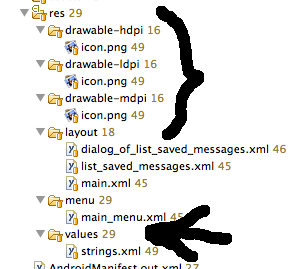
\includegraphics[scale=0.5]{img/estrutura.png}
		\end{figure}
    }
\section{Conclus�o}
   \frame
    {
        \frametitle{Refer�ncias}
        \begin{itemize}
            \item http://android-developers.blogspot.com/2009/04/backward-compatibility-for-android.html
            \item http://android-developers.blogspot.com/2010/07/how-to-have-your-cupcake-and-eat-it-too.html
            \item http://android-developers.blogspot.com/2010/06/making-sense-of-multitouch.html
        \end{itemize}
    }
\end{document}
